\begin{figure}[t]
\centering
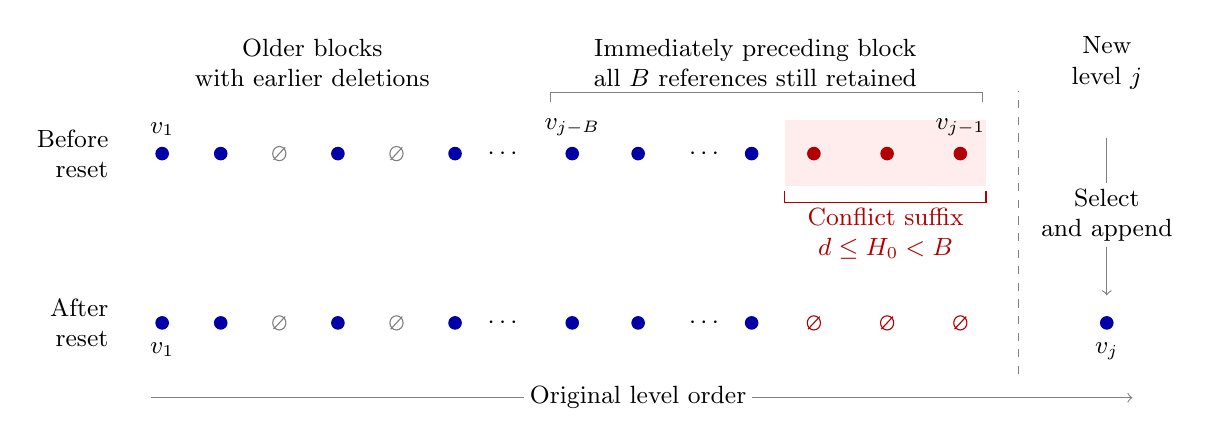
\begin{tikzpicture}[x=0.93cm,y=1cm,
  every node/.style={font=\small},
  kept/.style={circle,draw=blue!65!black,fill=blue!65!black,
               inner sep=0pt,minimum size=4.5pt},
  conflict/.style={circle,draw=red!70!black,fill=red!70!black,
                   inner sep=0pt,minimum size=4.5pt}]
  \node[align=center] at (3.35,3.45) {Older blocks\\with earlier deletions};
  \node[align=center] at (9.4,3.45)
      {Immediately preceding block\\all $B$ references still retained};
  \node[align=center] at (14.2,3.45) {New\\level $j$};
  \draw[gray] (6.6,2.96)--(6.6,3.08)--(12.5,3.08)--(12.5,2.96);
  \draw[gray,dashed] (13.0,-0.50)--(13.0,3.10);
  \node[anchor=east,align=right] at (0.7,2.30) {Before\\reset};
  \node[anchor=east,align=right] at (0.7,0.15) {After\\reset};

  \foreach \y in {2.30,0.15} {
    \foreach \x in {1.3,2.1,3.7,5.3}
      \node[kept] at (\x,\y) {};
    \foreach \x in {2.9,4.5} {
      \draw[gray] (\x,\y) circle[radius=0.09];
      \draw[gray] (\x-0.08,\y-0.08)--(\x+0.08,\y+0.08);
    }
    \node at (5.95,\y) {$\cdots$};
  }
  \node[above] at (1.3,2.40) {$v_1$};
  \node[below] at (1.3,0.02) {$v_1$};

  \fill[red!7] (9.80,1.89) rectangle (12.55,2.73);
  \foreach \x in {6.9,7.8}
    \node[kept] at (\x,2.30) {};
  \node at (8.7,2.30) {$\cdots$};
  \node[kept] at (9.35,2.30) {};
  \foreach \x in {10.2,11.2,12.2}
    \node[conflict] at (\x,2.30) {};
  \node[above] at (6.9,2.40) {$v_{j-B}$};
  \node[above] at (12.2,2.40) {$v_{j-1}$};
  \draw[red!70!black] (9.80,1.83)--(9.80,1.68)--(12.55,1.68)--(12.55,1.83);
  \node[text=red!70!black,align=center] at (11.18,1.28)
      {Conflict suffix\\$d\le H_0<B$};

  \foreach \x in {6.9,7.8,9.35}
    \node[kept] at (\x,0.15) {};
  \node at (8.7,0.15) {$\cdots$};
  \foreach \x in {10.2,11.2,12.2} {
    \draw[red!70!black] (\x,0.15) circle[radius=0.09];
    \draw[red!70!black] (\x-0.08,0.07)--(\x+0.08,0.23);
  }
  \node[kept] at (14.2,0.15) {};
  \node[below] at (14.2,0.02) {$v_j$};
  \draw[->,gray] (14.2,2.50)--(14.2,0.50);
  \node[align=center,fill=white,inner sep=2pt] at (14.2,1.52)
      {Select\\and append};

  \draw[->,gray] (1.15,-0.80)--(14.55,-0.80);
  \node[fill=white,inner sep=2pt] at (7.8,-0.80) {Original level order};
\end{tikzpicture}
\caption{Why a reset preserves the first reference. The dots are schematic
slots in the original level order; omitted entries are indicated by
ellipsis, and crossed gray slots represent deletions at earlier resets.
Immediately before a reset at level $j$, the preceding block
$\{j-B,\ldots,j-1\}$ is complete. Conflicts form a suffix of the retained
list of length $d\le H_0<B$, illustrated in red. The suffix therefore
misses both the first reference of that complete block and all older
retained references. Thus $v_1$ survives at the first reset, when it
belongs to the preceding block, and at every later reset, as drawn.
The new reference $v_j$ is then appended.
Older blocks may contain holes and need not be complete. The diagram
illustrates a nonempty conflict suffix; the proof also permits $d=0$.}
\label{fig:protected-block}
\end{figure}
